% ══════════════════════════════════════════════════════════════
% Copertina
% ══════════════════════════════════════════════════════════════
\begin{titlepage}
\thispagestyle{empty}
\begin{center}

\vspace*{0.5cm}
{\scshape\Large Università degli Studi di Napoli\\[2pt] Federico II\par}

\vspace{0.3cm}

% ── Logo (segnaposto automatico se il file non è presente) ──
\IfFileExists{Assets/logo_federico2.png}{%
    
\includegraphics[width=3.2cm]{Assets/logo_federico2.png}
}{%
    \fbox{\parbox[c][3.2cm][c]{3.2cm}{\centering\ttfamily\footnotesize
    Logo Federico~II\\ \vspace{2pt} \tiny(inserire \\ Assets/logo\_federico2.png)}}
}

\vspace{0.5cm}
{\scshape\large Dipartimento di Ingegneria Elettrica\\ e delle Tecnologie dell'Informazione (DIETI)\par}

\vspace{0.6cm}
{\scshape\large Corso di Laurea Magistrale in Informatica\par}
\vspace{0.15cm}
{\large Esame di Internet of Things\par}

\vspace{1.4cm}
{\Huge\bfseries PomodorIA\par}
\vspace{0.4cm}
{\Large Serra Domotica con Edge AI per il Riconoscimento\\ di Patologie Fogliari del Pomodoro\par}

\vspace{0.6cm}
{\large\itshape Proof of Concept software --- simulazione end-to-end\\ del ciclo \emph{sense-think-act} su un dispositivo Edge simulato\par}

\vspace{0.8cm}
{\normalsize Anno Accademico: 2025/2026\par}

\vfill

% ── Riga finale: autori a sinistra, immagine di copertina a destra ──
\begin{minipage}[b]{0.55\textwidth}
    \raggedright
    \textbf{Autori}\\[4pt]
    Gianmarco Vellotti \quad N\textsuperscript{o} matricola: \emph{da completare}\\
    Francesco Terrecuso \quad N\textsuperscript{o} matricola: \emph{da completare}\\[10pt]
    \textbf{Docente}\\[4pt]
    Prof. Silvio Barra
\end{minipage}
\hfill
\begin{minipage}[b]{0.38\textwidth}
    \raggedleft
    \IfFileExists{Assets/cover_image.jpg}{%
        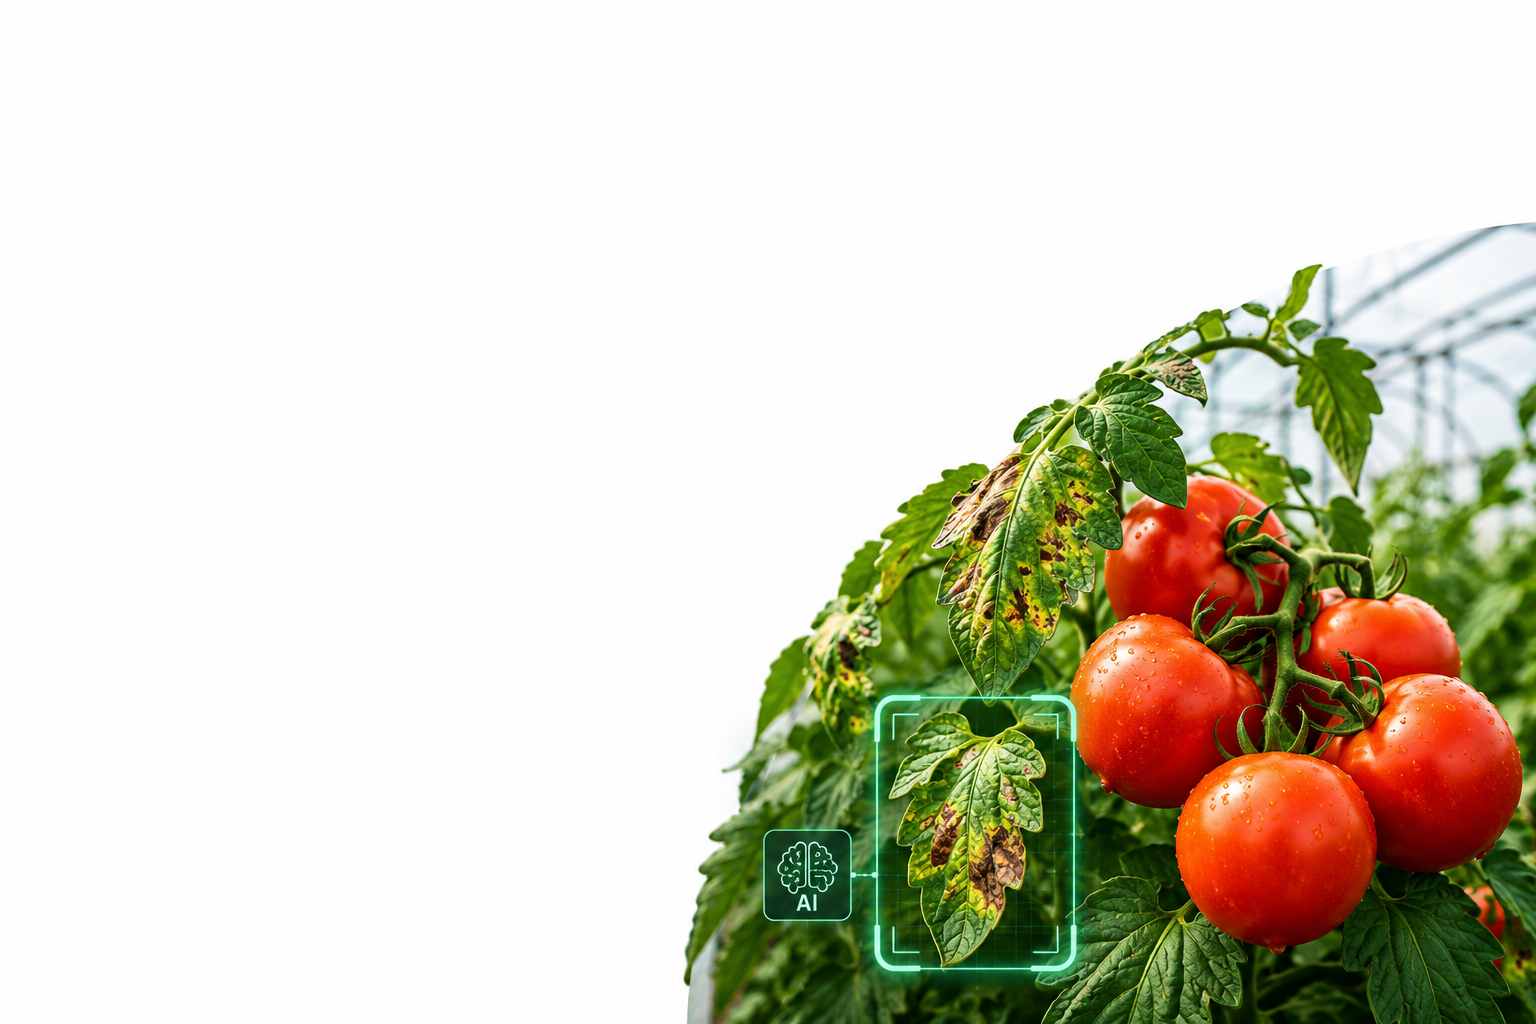
\includegraphics[width=\textwidth]{Assets/cover_image.jpg}
    }{%
        \fbox{\parbox[c][3.4cm][c]{0.95\textwidth}{\centering\ttfamily\footnotesize
        Immagine di copertina\\ \vspace{2pt}\tiny(inserire Assets/cover\_image.jpg\\
        --- es. foglia di pomodoro / serra)}}
    }
\end{minipage}

\vspace{0.4cm}

\end{center}
\end{titlepage}
